%!TEX program = xelatex
%% Copyright (C) 2025 傅祉珏
%% 
%% This file contains LaTeX source code for the Homework1 of YatRL,
%% released under AGPLv3 license.
%% Full license text available in LICENSE file at project root,
%% with additional restrictions in ADDITIONAL_TERMS.md.
%% 
%% Commercial use prohibited. Academic use requires retention of this notice.
%% Source repository: https://github.com/Billiefu/YatRL

% SPDX-FileCopyrightText: 2025 傅祉珏
% SPDX-License-Identifier: AGPL-3.0-or-later
% SPDX-Additional-Clauses: see ADDITIONAL_TERMS.md

\documentclass[a4paper, utf8]{ctexart}
\usepackage[fontset=Fandol]{ctex}
\usepackage{draftwatermark}
\usepackage{algpseudocode}
\usepackage{algorithmicx}
\usepackage{anyfontsize}
\usepackage{subcaption}
\usepackage{algorithm}
\usepackage{abstract}
\usepackage{amsfonts}
\usepackage{appendix}
\usepackage{enumitem}
\usepackage{fancyhdr}
\usepackage{fontspec}
\usepackage{geometry}
\usepackage{graphicx}
\usepackage{amsmath}
\usepackage{caption}
\usepackage{lipsum}
\usepackage{minted}
\usepackage{url}

\usepackage{tikz}
\usetikzlibrary{arrows.meta, positioning}
\usepackage{amsmath}

\setsansfont{Latin Modern Roman}
\geometry{a4paper,left=25mm,right=25mm,top=25mm,bottom=25mm}
\CTEXsetup[format={\Large \bfseries}]{section}
\setlength{\parindent}{2em}
\pagestyle{fancy}
\fancyhf{}

\fancyhead[C]{}
\fancyhead[L]{HOMEWORK1:\ Grid\ Maze\ Solver}
\fancyhead[R]{21307210\ 傅祉珏}
\fancyfoot[C]{\thepage}
\fancyfoot[L,R]{}

\renewcommand{\figurename}{Fig}
\renewcommand{\refname}{References}
\renewcommand{\tablename}{Table}

\title{\songti \Large \textbf{HOMEWORK1:\ Grid\ Maze\ Solver}}
\author{傅祉珏 \quad 21307210}
\date{\fangsong Sun Yat-sen University, School of Computer Science and Engineering}

\SetWatermarkText{}
\SetWatermarkText{Copyright\ \copyright\ 2025\ 傅祉珏}
\SetWatermarkScale{0.4}
\SetWatermarkAngle{45}
\SetWatermarkColor[gray]{0.8}

\begin{document}

	\begin{titlepage}
		\centering
		\rule{\textwidth}{1pt}
		\vspace{0.02\textheight}
		
		{\LARGE \kaishu YatRL \quad SYSU\ CSE\ 2025-1 \quad Homework1}
		
		\vspace{0.02\textheight}
		
		{\Huge \songti \bfseries Grid\ Maze\ Solver}
		
		\vspace{0.025\textheight}
		\rule{0.83\textwidth}{0.4pt}
		\vspace{0.05\textheight} 
		\begin{figure}[htbp]
			\centering
			\includegraphics[width=8cm, height=8cm]{./figure/计院院徽.jpg}
		\end{figure}
		
		\vspace{0.05\textheight}
        {\Large Course Number:\textsc{DCS245}}

        \vspace{0.025\textheight}
        {\Large Student's Name:\textsc{傅祉珏}}

        \vspace{0.025\textheight}
        {\Large Student's Number:\textsc{21307210}}

        \vspace{0.025\textheight}
        {\Large Advisor's Name / Title:\textsc{Prof. Chen Xu}}

        \vspace{0.025\textheight}
        {\Large Date Due:\textsc{30 October, 2025}}
		
		\vspace{0.05\textheight} 
		\vfill
		
		{\large 21 October, 2025}
		\vspace{0.1\textheight}
		\rule{\textwidth}{1pt}
	\end{titlepage}
	\let\cleardoublepage\clearpage
	
	\maketitle
	
	\renewcommand{\abstractname}{\large \textbf{Abstract}}
	\begin{abstract}
		This report aims to deeply investigate and implement dynamic programming algorithms based on the Markov Decision Process (MDP) to solve the classic grid maze path planning problem. In this work, we first rigorously formalize the maze environment as an MDP model, explicitly defining its states, actions, transition probabilities, and reward function. Subsequently, we implement three core dynamic programming algorithms: Value Iteration, Policy Iteration, and Truncated Policy Iteration, a hybrid of the two, and apply them to solve maze scenarios of varying complexities within a Python programming environment. The experimental results demonstrate that all algorithms successfully converge to and identify the optimal policy from the start to the goal. More importantly, this study reveals through comparative analysis that there is no fixed performance hierarchy among the three algorithms; their convergence efficiency is closely related to the specific structure and scale of the problem. Notably, in a maze of medium complexity, Value Iteration anomalously converges faster than Truncated Policy Iteration, a phenomenon that reveals Truncated Policy Iteration may fall into a suboptimal policy trap under certain conditions due to its 'myopic' evaluation. This research not only validates the effectiveness of dynamic programming algorithms but also provides a profound, practical insight into their respective internal mechanisms, performance trade-offs, and applicable scenarios, offering valuable guidance for selecting and optimizing decision-making algorithms in real-world problems. The complete source code is available at \url{https://github.com/Billiefu/YatRL2025.git}.
		
		\noindent{\textbf{\heiti Key words:}Reinforcement Learning; Markov Decision Process; Dynamic Programming; Value Iteration; Policy Iteration; Path Planning.}
	\end{abstract}
	
	\section{Introduction}
	
	With the rapid development of computational power, Reinforcement Learning (RL), as a significant branch of artificial intelligence, has become a key theoretical framework for solving complex sequential decision-making problems. The core idea of RL is to enable an agent to learn through direct interaction with an environment. In a continuous process of trial and error, the agent adjusts its behavioral policy based on the rewards or punishments received as feedback from the environment, with the ultimate goal of learning an optimal policy that maximizes long-term cumulative rewards. This learning paradigm, originating from behavioral psychology, has demonstrated immense application potential in numerous frontier domains, including robotics control, autonomous driving, and medical diagnostics.
    
    To provide a rigorous mathematical model for sequential decision-making problems, the Markov Decision Process (MDP) is commonly used for formal description; a standard reinforcement learning task is essentially an MDP. An MDP is constituted by a set of key elements, including a set of states, a set of actions, state transition probabilities, and a reward function. In this study, we model the classic grid maze problem as an MDP. Here, each position of the agent in the maze corresponds to a state, and the "up, down, left, right" movements it can perform are the actions. The environment model is defined as deterministic, where the agent receives a fixed negative reward for each step taken, thereby incentivizing it to discover the shortest path from the start to the goal.
    
    When the environmental model of a problem is fully known—that is, the agent has complete knowledge of the state transition probabilities and reward function—Dynamic Programming (DP) becomes an efficient method for finding the optimal policy. Among the various DP algorithms, Policy Iteration and Value Iteration are two foundational and classic algorithms. Value Iteration directly approximates the optimal state-value function by repeatedly iterating the Bellman optimality equation, from which the optimal policy is then derived. In contrast, Policy Iteration continuously refines the current policy by alternating between two steps, "policy evaluation" and "policy improvement," until convergence is achieved.
    
    This paper aims to systematically solve a specific grid maze problem. We will first rigorously model this problem as a Markov Decision Process, and subsequently apply Value Iteration, Policy Iteration, and its hybrid form, Truncated Policy Iteration, to solve for the optimal value function and optimal policy under this MDP. Finally, we will present and conduct an in-depth analysis of the experimental results, not only to validate the effectiveness of the algorithms but also to uncover the performance differences and underlying mechanisms of these algorithms under specific problem structures.
	
	\section{Related Work}
	
	As the core framework for solving sequential decision-making problems, the development of Reinforcement Learning's theory and algorithms is built upon decades of research accumulation. The grid maze problem we currently aim to solve is essentially a search for an optimal policy in a fully known environment, a classic problem that is a direct application of Markov Decision Process (MDP) theory. MDPs provide a rigorous mathematical formalization for such problems, enabling us to systematically analyze and solve for the optimal path. In recent years, numerous scholars have systematically reviewed and summarized the foundational theories, cutting-edge research, and practical applications of RL, providing a solid theoretical foundation for our understanding of core concepts like MDPs and dynamic programming.
    
    Based on the MDP model, when the dynamics of the environment (i.e., the state transition probabilities and reward function) are known, dynamic programming is the preferred method for finding the optimal policy. Among these, Value Iteration and Policy Iteration are two of the most foundational algorithms. As early as 1996, Pashenkova et al. conducted in-depth research and comparison of these two core algorithms, providing theoretical guidance for selecting appropriate solution methods for different types of MDP problems. These early works established the fundamental paradigm of approximating the optimal solution by iteratively computing value functions or directly optimizing policies, forming the core algorithmic basis upon which our current work relies.
    
    As research progressed, scholars were not limited to the standard MDP model but also extended and deepened it. For instance, Whitehead and Lin explored methods for reinforcement learning in non-Markov decision processes in 1995, broadening the application boundaries of RL. Szepesvári and Littman proposed generalized Markov decision processes and discussed corresponding dynamic programming and reinforcement learning algorithms, further enriching the theoretical system of sequential decision-making. Concurrently, to enhance the efficiency of classical algorithms, researchers have proposed various improvements. The Truncated Policy Iteration method, introduced by Dembo and Haviv in 1984, effectively combines the advantages of Value Iteration and Policy Iteration by performing a finite number of iterations in the policy evaluation step, providing a new approach to accelerate algorithm convergence.
    
    The value of these theories and algorithms is not only reflected in academic research but has also been validated in numerous practical application domains. For example, Wei et al. successfully applied the MDP framework to the learning-to-rank task in information retrieval, constructing a reinforcement ranking model and demonstrating the great potential of MDPs as a powerful tool for solving complex real-world problems.
	
	\section{Method}
	
	This research aims to solve a classic Grid Maze problem, the core of which is to find the optimal path from a start point to a goal. Given that this problem possesses well-defined states, actions, and deterministic state transition and reward mechanisms, we model it as a Markov Decision Process (MDP). Since the environment model is completely known, Dynamic Programming (DP) is the ideal method for solving such problems. This study will be based on the Bellman equation and will employ and compare three classic dynamic programming algorithms: Value Iteration, Policy Iteration, and its hybrid form, Truncated Policy Iteration, to solve for the optimal policy.

    Dynamic Programming is an optimization algorithm originating from the field of optimal control, used to solve multi-stage sequential decision-making problems. Its core idea is to decompose a complex problem into a series of simpler subproblems, solve and store the optimal solutions to these subproblems, and ultimately combine them to form the optimal solution to the original problem. DP methods require the environment model to be known, meaning the agent has complete knowledge of the state transitions and rewards resulting from any action.

    \subsection{The Bellman Equation}

    The theoretical cornerstone for solving MDPs with dynamic programming is the Bellman Equation. This equation recursively defines the state-value function $v^\pi(s)$ -- that is, the expected discounted return achievable from state $s$ by following policy $\pi$.

    \vspace{-.5em}
    \begin{equation}
        v^\pi(s)=\mathbb{E}_\pi[G_t|S_t=s]=\sum_{a\in A}\pi(a|s)\sum_{s'\in S}P(s'|s,a)[r(s,a,s')+\gamma v^\pi(s')]
    \end{equation}

    Here, $\pi(a|s)$ is the policy function, which represents the probability of selecting action $a$ in state $s$; $P(s'|s,a)$ is the state transition probability; $r(s,a,s')$ is the immediate reward; and $\gamma$ is the discount factor.

    However, our ultimate goal is not to evaluate an arbitrary policy, but to find an optimal policy $\pi^*$ whose value function $v^*(s)$ is superior or equal to that of any other policy for all states. This optimal value function adheres to the Bellman Optimality Equation, which embodies the principle of optimality by introducing a $\max$ operator.

    \vspace{-.5em}
    \begin{equation}
        v^*(s)=\max\limits_{a\in A}\sum_{s'\in S}P(s'|s,a)[r(s,a,s')+\gamma v^*(s')]
    \end{equation}

    The Bellman optimality equation states that the value of a state under an optimal policy is equal to the expected return achievable by taking the optimal action in that state. The algorithms to be introduced subsequently are all essentially methods for effectively solving this equation.

    \subsection{Value Iteration}

    The Value Iteration (VI) algorithm is a process that approximates the optimal value function $v^*(s)$ by iteratively updating the state-value function. Its core idea is to directly use the Bellman optimality equation as the update rule. This algorithm merges the steps of policy improvement and value update into a single iteration.

    \vspace{-.5em}
    \begin{equation}
        v_{k+1}(s) = \max_{a \in A} \sum_{s' \in S} P(s'|s,a)[r(s,a,s') + \gamma v_k(s')]
    \end{equation}

    In each iteration, the algorithm computes the new value $v_{k+1}(s)$ for all states $s$ in parallel. This process implicitly performs one step of policy improvement (by selecting the optimal action via the $\max$ operation) and one step of policy evaluation (by using the old value function $v_k$ to calculate the new value). The iteration stops when the value function converges, i.e., when $\max_s\left\| v_{k+1}(s)-v_k(s) \right\|$ is less than a preset threshold. Finally, the optimal policy $\pi^*$ can be easily extracted from the converged value function $v^*$.

    \vspace{-.5em}
    \begin{equation}
        \pi^*(s) = \arg\max_{a \in A} \sum_{s' \in S} P(s'|s,a)[r(s,a,s') + \gamma v^*(s')]
    \end{equation}

    \subsection{Policy Iteration}

    The Policy Iteration (PI) algorithm, in contrast, performs a direct search in the policy space. It starts with an initial policy $\pi_0$ and alternates between two steps, "policy evaluation" and "policy improvement," until the policy no longer changes.

    The first step is Policy Evaluation. For the current policy $\pi_k$, we need to accurately compute its corresponding state-value function $v_{\pi_k}$. This is achieved by iteratively solving the Bellman expectation equation.

    \vspace{-.5em}
    \begin{equation}
    v^{(j+1)}_{\pi_k}(s) = \sum_{a \in A} \pi_k(a|s) \sum_{s' \in S} P(s'|s,a)[r(s,a,s') + \gamma v^{(j)}_{\pi_k}(s')]
    \end{equation}

    The second step is Policy Improvement. Based on the evaluated value function $v^{(j)}_{\pi_k}$, we update the policy using a greedy strategy to generate the new policy $\pi_{k+1}$.

    \vspace{-.5em}
    \begin{equation}
        \pi_{k+1}(s) = \arg\max_{a \in A} \sum_{s' \in S} P(s'|s,a)[r(s,a,s') + \gamma v_{\pi_k}(s')]
    \end{equation}

    These two steps are repeated alternately until the policy $\pi_{k+1}$ is identical to $\pi_k$. At this point, the algorithm has converged, having found the optimal policy and the optimal value function.

    \subsection{Truncated Policy Iteration}

    By comparison, it is evident that Value Iteration performs only a single Bellman update per iteration (equivalent to one incomplete policy evaluation), whereas Policy Iteration requires the value function to be iterated until full convergence during its policy evaluation phase. The Truncated Policy Iteration (TPI) algorithm is a compromise that lies between these two extremes.

    \vspace{1em}
    \begin{center}
        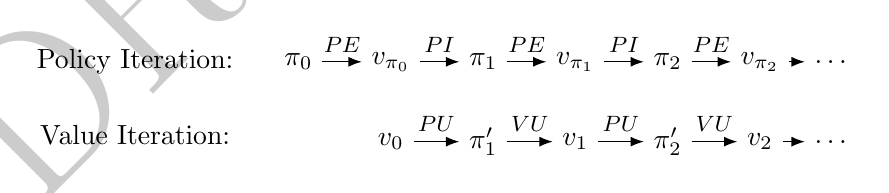
\begin{tikzpicture}[
            node distance=0.5cm and 0.5cm,
            box/.style={rectangle, minimum width=0.5cm, minimum height=0.6cm, align=center},
            arrow/.style={-Latex, thin},
            label/.style={font=\small}
        ]
            \node[align=right] (PI_Title) {Policy Iteration:};
            \node[box, right=0.4cm of PI_Title] (pi0) {$\pi_0$};
            \node[box, right=of pi0] (vpi0) {$v_{\pi_0}$};
            \node[box, right=of vpi0] (pi1) {$\pi_1$};
            \node[box, right=of pi1] (vpi1) {$v_{\pi_1}$};
            \node[box, right=of vpi1] (pi2) {$\pi_2$};
            \node[box, right=of pi2] (vpi2) {$v_{\pi_2}$};
            \node[box, right=0.2cm of vpi2] (dots_pi) {$\dots$};
            \draw[arrow] (pi0) -- node[above, label] {\footnotesize $PE$} (vpi0);
            \draw[arrow] (vpi0) -- node[above, label] {\footnotesize $PI$} (pi1);
            \draw[arrow] (pi1) -- node[above, label] {\footnotesize $PE$} (vpi1);
            \draw[arrow] (vpi1) -- node[above, label] {\footnotesize $PI$} (pi2);
            \draw[arrow] (pi2) -- node[above, label] {\footnotesize $PE$} (vpi2);
            \draw[arrow] (vpi2) -- (dots_pi);
            
            \node[align=right, below=0.4cm of PI_Title] (VI_Title) {Value Iteration:};
            \node[box, below=0.4cm of vpi0] (v0) {$v_0$};
            \node[box, below=0.4cm of pi1] (pi1prime) {$\pi'_1$};
            \node[box, below=0.4cm of vpi1] (v1) {$v_1$};
            \node[box, below=0.4cm of pi2] (pi2prime) {$\pi'_2$};
            \node[box, below=0.4cm of vpi2] (v2) {$v_2$};
            \node[box, below=0.4cm of dots_pi] (dots_vi) {$\dots$};
            \draw[arrow] (v0) -- node[above, label] {\footnotesize $PU$} (pi1prime);
            \draw[arrow] (pi1prime) -- node[above, label] {\footnotesize $VU$} (v1);
            \draw[arrow] (v1) -- node[above, label] {\footnotesize $PU$} (pi2prime);
            \draw[arrow] (pi2prime) -- node[above, label] {\footnotesize $VU$} (v2);
            \draw[arrow] (v2) -- (dots_vi);
        \end{tikzpicture}
    \end{center}
    \vspace{1em}

    The structure of this algorithm is similar to that of Policy Iteration, also comprising policy evaluation and policy improvement stages. The key difference lies in its policy evaluation step, which does not iterate until full convergence but instead runs for a fixed, smaller number of iterations, $m$. This "incomplete evaluation" significantly reduces the computational cost per iteration while providing richer value information than the single-step update of Value Iteration. By striking a balance between computational efficiency and evaluation accuracy, Truncated Policy Iteration can often outperform the other two algorithms in terms of total computation time, especially in problems with large state spaces. When the truncation depth $m=1$, this algorithm is equivalent to Value Iteration; as $m\rightarrow\infty$, it becomes equivalent to Policy Iteration.
	
	\section{Experiments}

    \begin{figure}[t]
        \centering
        \begin{subfigure}{.4\textwidth}
            \centering
            \includegraphics[height=.2\textheight]{figure/e1-value.png}
            \caption{Final State Values of Different States}
        \end{subfigure}
        \begin{subfigure}{.5\textwidth}
            \centering
            \includegraphics[height=.2\textheight]{figure/e1-curve.png}
            \caption{Convergence Curves of Different Algorithms}
        \end{subfigure}
        \caption{Experimental Results of the Given Maze ($8\times8$)}
    \end{figure}
	
	To deeply investigate the dynamic characteristics and performance differences of Value Iteration, Policy Iteration, and its variant, Truncated Policy Iteration, during the actual solution process, we designed and executed a series of experiments. All experiments were based on a unified reinforcement learning environment where an agent explores a discrete grid maze. This environment was modeled as a deterministic Markov Decision Process, in which the agent receives a penalty of $-1$ for each move until it reaches the goal, which has a reward of $0$. This reward structure is designed to compel the algorithms to find the shortest path. In all tests, we uniformly used a discount factor of $0.9$ to balance long-term benefits, set a convergence precision threshold of $1e-6$, and fixed the internal evaluation depth of Truncated Policy Iteration to 5 sweeps.

    Our core investigation began with the standard $8\times8$ maze specified in the assignment. Initial results showed that all three algorithms performed excellently, successfully converging to and computing the exact same optimal policy, which clearly marked a direct path from the start to the goal without detours. The heatmap of the final converged value function visually corroborated this, with values smoothly decreasing from zero at the goal towards the outer states, accurately reflecting the cost of the shortest distance from each point to the goal, thus validating the correctness of all algorithms' solutions.
    
    However, when we shifted our analysis to the convergence process, an anomalous phenomenon contrary to common theory emerged. In the test on the standard maze, the Value Iteration algorithm converged in just 23 iterations, a speed significantly superior to Truncated Policy Iteration, which required 19 outer iterations (each containing 5 inner evaluation sweeps). The convergence curve of the starting state's value clearly shows that Truncated Policy Iteration's performance curve was stuck in a low-value plateau for an extended initial period, only "awakening" and rapidly approaching the optimal value after the 14th outer iteration.
    
    To uncover the underlying mechanism of this anomaly, we conducted a visual snapshot analysis of the value function's evolution. The analysis revealed that the root of the problem lies in the coupling of Truncated Policy Iteration's "myopic" evaluation mechanism with the specific topology of this maze. In the initial phase, the algorithm performs its evaluation based on a randomly generated, suboptimal policy. Because the truncated evaluation consists of only 5 inner sweeps, this is insufficient for the true value information from the goal to fully propagate back to decision nodes deep within the maze. Consequently, the algorithm improves its policy based on this incomplete and misleading value assessment, thereby falling into a "locally optimal" policy trap. It requires the cumulative effect of many outer iterations to gradually correct this early mistake. In stark contrast, Value Iteration does not rely on any explicit policy; its value updates spread steadily outwards like ripples from a center, making the process robust and predictable. In this medium-sized maze, this policy-unconstrained propagation method paradoxically surpassed the misguided Truncated Policy Iteration.

    \begin{figure}[t]
        \centering
        \begin{subfigure}{.4\textwidth}
            \centering
            \includegraphics[height=.2\textheight]{figure/e2-value.png}
            \caption{Final State Values of Different States}
        \end{subfigure}
        \begin{subfigure}{.5\textwidth}
            \centering
            \includegraphics[height=.2\textheight]{figure/e2-curve.png}
            \caption{Convergence Curves of Different Algorithms}
        \end{subfigure}
        \caption{Experimental Results of the Given Maze ($21\times21$)}
    \end{figure}
    
    To validate this hypothesis, we further extended our experiments to a structurally simpler $5\times5$ maze and a highly complex $21\times21$ maze. The results strongly supported our analysis: in the simple maze, due to the small state space, 5 sweeps of truncated evaluation were nearly equivalent to a full evaluation, making the behavior of Truncated Policy Iteration indistinguishable from the highly efficient Policy Iteration, leading to rapid convergence. Conversely, in the complex $21\times21$ maze, the theoretical performance ranking was perfectly reproduced—Value Iteration was the slowest to converge due to its point-wise update nature, while Truncated Policy Iteration fully leveraged its advantage as an efficient compromise, converging much faster than Value Iteration and ranking solidly behind Policy Iteration.

    \begin{figure}[t]
        \centering
        \begin{subfigure}{.4\textwidth}
            \centering
            \includegraphics[height=.2\textheight]{figure/e3-value.png}
            \caption{Final State Values of Different States}
        \end{subfigure}
        \begin{subfigure}{.5\textwidth}
            \centering
            \includegraphics[height=.2\textheight]{figure/e3-curve.png}
            \caption{Convergence Curves of Different Algorithms}
        \end{subfigure}
        \caption{Experimental Results of the Given Maze ($5\times5$)}
    \end{figure}
    
    In summary, our experiments not only demonstrated the effectiveness of dynamic programming algorithms for path planning problems but also, through an in-depth analysis of an anomalous experimental phenomenon, revealed that algorithm performance is not static. Instead, it is a complex result of the interaction between an algorithm's internal mechanisms and the specific structure of the problem. The efficiency of Truncated Policy Iteration is highly dependent on whether its truncation depth is sufficient to provide insight into the problem's critical decision points, which offers profound implications for selecting and tuning algorithms in practical applications.
	
	\section{Conclusion}
	
	Through the solution and analysis of the grid maze problem, we conclude that there is no simple linear performance ranking among Value Iteration, Policy Iteration, and Truncated Policy Iteration. Instead, their relationship is a dynamic and interconnected trade-off. Value Iteration forms the bedrock of algorithmic robustness; its policy-unconstrained value propagation mechanism ensures stable convergence in environments of any structure. Policy Iteration represents the theoretical optimum in terms of iteration count, trading immense per-step computational cost for the fewest policy updates. As a bridge between the two, Truncated Policy Iteration's performance is highly dependent on the effectiveness of the information provided by its "incomplete evaluation," making it a leader in efficiency in most cases (especially for large-scale problems), but also exposing its risk of falling into local optima in certain problem structures.
    
    This conclusion offers new perspectives and future directions for algorithmic performance optimization. Since each of the three algorithms has its own domain of advantage, future research could focus on how to dynamically and adaptively combine their strengths. For instance, one could design an adaptive truncated policy iteration algorithm capable of online monitoring of the "stagnation" degree of policy improvement. When slow convergence is detected (potentially indicating a suboptimal trap), the algorithm could automatically increase its internal evaluation depth to perform a more precise "deep evaluation" to escape the trap, reverting to a shallower evaluation depth during smooth convergence to maintain efficiency.
    
    Furthermore, hybrid algorithms based on a Value Iteration "warm start" could be explored. Specifically, one could first run a few computationally inexpensive iterations of Value Iteration to quickly generate a rough but reasonable initial estimate of the value function for the entire state space. Subsequently, this value function, which is far superior to a "zero-initialization," can be used as the starting point for Policy Iteration or Truncated Policy Iteration. This "warm start" approach is expected to significantly reduce the convergence time of the subsequent algorithms and, in particular, can effectively mitigate the risk of Truncated Policy Iteration being led astray by a random policy in its initial phase. The design of these adaptive and hybrid strategies means no longer viewing each algorithm in isolation, but rather as components of a toolbox to be intelligently combined based on real-time feedback from the problem. This approach promises to achieve a superior combination of computational efficiency and convergence stability across a broader range of complex decision-making problems.
	
	\let\cleardoublepage\clearpage
	
	\begin{thebibliography}{99}  
		\bibitem{ref1} 董豪, 丁子涵, 仉尚航等. 深度强化学习: 基础、研究与应用[M]. 第1版. 北京:电子工业出版社, 2021.
        \bibitem{ref2} 张伟楠, 沈键, 俞勇. 动手学强化学习[M]. 第1版. 北京:人民邮电出版社, 2022.
        \bibitem{ref3} 赵世钰. 强化学习的数学原理[M]. 第1版. 北京:清华大学出版社, 2025.
        \bibitem{ref4} 赵世钰. 强化学习的数学原理:英文[M]. 第1版. 北京:清华大学出版社, 2024.
        \bibitem{ref5} Dembo R S, Haviv M. Truncated policy iteration methods[J]. Operations research letters, 1984, 3(5): 243-246.
        \bibitem{ref6} Pashenkova E, Rish I, Dechter R. Value iteration and policy iteration algorithms for Markov decision problem[C]//AAAI’96: Workshop on Structural Issues in Planning and Temporal Reasoning. Citeseer. 1996.
        \bibitem{ref7} Szepesvári C, Littman M L. Generalized markov decision processes: Dynamic-programming and reinforcement-learning algorithms[C]//Proceedings of International Conference of Machine Learning. 1996, 96.
        \bibitem{ref8} Wei Z, Xu J, Lan Y, et al. Reinforcement learning to rank with Markov decision process[C]//Proceedings of the 40th international ACM SIGIR conference on research and development in information retrieval. 2017: 945-948.
        \bibitem{ref9} Whitehead S D, Lin L J. Reinforcement learning of non-Markov decision processes[J]. Artificial intelligence, 1995, 73(1-2): 271-306.
	\end{thebibliography}
    \newpage

    \appendix
	{\centering{\Large{\textbf{Appendix}}}}
    
    \section{Pseudocode for Different Algorithms}

    \begin{algorithm}[H]
        \caption{Value Iteration Algorithm}
        \begin{algorithmic}[1]
            \Require All probability models and state-action pairs are known, with a specified initial value function $v_0$
            \Ensure Find the optimal state value and policy that solve the Bellman optimality equation
            \While {$v_k$ has not converged, i.e., $\left\| v_k-v_{k-1} \right\|$ is greater than a desired threshold}
            \For{$\forall s \in S$}
            \For{$\forall a \in A$}
            \State Q-value: $q_k(s,a)=\sum_{s'}P(s'|s,a)r(s,s')+\gamma\sum_{s'}P(s'|s,a)v_k(s')$
            \EndFor
            \State Get action with max value: $a^*_k(s)=\arg\max_a q_k(s,a)$
            \State Policy update: $\pi_{k+1}(a|s)=1$ if $a=a^*_k(s)$; otherwise $\pi_{k+1}(a|s)=0$
            \State Value update: $v_{k+1}(s)=\max_a q_k(s,a)$
            \EndFor
            \EndWhile
        \end{algorithmic}
    \end{algorithm}

    \begin{algorithm}[H]
        \caption{Policy Iteration Algorithm}
        \begin{algorithmic}[1]
            \Require All probability models and state-action pairs are known, with a specified initial policy $\pi_0$
            \Ensure Find the optimal state value and policy
            \While {policy has not converged}
            \While {$v^{(j)}_{\pi_k}$ has not converged}
            \For{$\forall s \in S$}
            \State $v^{(j+1)}_{\pi_k}(s)=\sum_a\pi_k(a|s)\sum_{s'}P(s'|s,a)\left( r(s,s')+\gamma v^{(j)}_{\pi_k}(s') \right)$
            \EndFor
            \EndWhile
            \For{$\forall s \in S$}
            \For{$\forall a \in A$}
            \State Q-value: $q_{\pi_k}(s,a)=\sum_{s'}P(s'|s,a)r(s,s')+\gamma\sum_{s'}P(s'|s,a)v_{\pi_k}(s')$
            \EndFor
            \State $a^*_k(s)=\arg\max_a q_{\pi_k}(s,a)$
            \State $\pi_{k+1}(a|s)=1$ if $a=a^*_k(s)$; otherwise $\pi_{k+1}(a|s)=0$
            \EndFor
            \EndWhile
        \end{algorithmic}
    \end{algorithm}

    \begin{algorithm}[H]
        \caption{Truncated Policy Iteration Algorithm}
        \begin{algorithmic}[1]
            \Require All probability models and state-action pairs are known, with a specified initial policy $\pi_0$
            \Ensure Find the optimal state value and policy
            \While {policy has not converged}
            \State Initialize a state value estimate $v^{(0)}_k=v_{k-1}$, and set the max number of iterations to $j_{truncate}$
            \While {$j<j_{truncate}$}
            \For{$\forall s \in S$}
            \State $v^{(j+1)}_{k}(s)=\sum_a\pi_k(a|s)\sum_{s'}P(s'|s,a)\left( r(s,s')+\gamma v^{(j)}_{k}(s') \right)$
            \EndFor
            \EndWhile
            \State Set $v_k=v^{(j_{truncate})}_k$
            \For{$\forall s \in S$}
            \For{$\forall a \in A$}
            \State Q-value: $q_{\pi_k}(s,a)=\sum_{s'}P(s'|s,a)r(s,s')+\gamma\sum_{s'}P(s'|s,a)v_{k}(s')$
            \EndFor
            \State $a^*_k(s)=\arg\max_a q_{\pi_k}(s,a)$
            \State $\pi_{k+1}(a|s)=1$ if $a=a^*_k(s)$; otherwise $\pi_{k+1}(a|s)=0$
            \EndFor
            \EndWhile
        \end{algorithmic}
    \end{algorithm}

    \section{Intermediate Results of Different Algorithms}

    \begin{figure}[H]
        \centering
        \begin{subfigure}{.95\textwidth}
            \centering
            \includegraphics[width=\textwidth]{figure/e1-vi.png}
            \caption{Convergence Process of Value Iteration}
        \end{subfigure}
    \end{figure}
    \begin{figure}[H]
        \ContinuedFloat
        \centering
        \begin{subfigure}{.95\textwidth}
            \centering
            \includegraphics[width=\textwidth]{figure/e1-pi.png}
            \caption{Convergence Process of Policy Iteration}
        \end{subfigure}
    \end{figure}
    \begin{figure}[H]
        \ContinuedFloat
        \centering
        \begin{subfigure}{.95\textwidth}
            \centering
            \includegraphics[width=\textwidth]{figure/e1-tpi.png}
            \caption{Convergence Process of Truncated Policy Iteration}
        \end{subfigure}
        \caption{Visualization of the Convergence Process of A Given Maze ($8\times8$)}
    \end{figure}

    \begin{figure}[H]
        \centering
        \begin{subfigure}{.95\textwidth}
            \centering
            \includegraphics[width=\textwidth]{figure/e2-vi.png}
            \caption{Convergence Process of Value Iteration}
        \end{subfigure}
    \end{figure}
    \begin{figure}[H]
        \ContinuedFloat
        \centering
        \begin{subfigure}{.95\textwidth}
            \centering
            \includegraphics[width=\textwidth]{figure/e2-pi.png}
            \caption{Convergence Process of Policy Iteration}
        \end{subfigure}
    \end{figure}
    \begin{figure}[H]
        \ContinuedFloat
        \centering
        \begin{subfigure}{.95\textwidth}
            \centering
            \includegraphics[width=\textwidth]{figure/e2-tpi.png}
            \caption{Convergence Process of Truncated Policy Iteration}
        \end{subfigure}
        \caption{Visualization of the Convergence Process of A Given Maze ($21\times21$)}
    \end{figure}

    \begin{figure}[H]
        \centering
        \begin{subfigure}{.95\textwidth}
            \centering
            \includegraphics[width=\textwidth]{figure/e3-vi.png}
            \caption{Convergence Process of Value Iteration}
        \end{subfigure}
    \end{figure}
    \begin{figure}[H]
        \ContinuedFloat
        \centering
        \begin{subfigure}{.95\textwidth}
            \centering
            \includegraphics[width=\textwidth]{figure/e3-pi.png}
            \caption{Convergence Process of Policy Iteration}
        \end{subfigure}
    \end{figure}
    \begin{figure}[H]
        \ContinuedFloat
        \centering
        \begin{subfigure}{.95\textwidth}
            \centering
            \includegraphics[width=\textwidth]{figure/e3-tpi.png}
            \caption{Convergence Process of Truncated Policy Iteration}
        \end{subfigure}
        \caption{Visualization of the Convergence Process of A Given Maze ($5\times5$)}
    \end{figure}
	
\end{document}
